\documentclass[12pt]{article}


\usepackage{amssymb}
\usepackage{amsmath}
\usepackage{fullpage}
\usepackage{epsfig}
\usepackage{epstopdf}
\everymath{\displaystyle}



\begin{document}

\begin{center}
\underline{\LARGE{Chapter 2.5 Practice Problems}}
\end{center}

\noindent EXPECTED SKILLS:

\begin{itemize}

\item Know the derivatives of the 6 elementary trigonometric functions.

\item Be able to use these derivatives in the context of word problems.

\end{itemize}

\noindent PRACTICE PROBLEMS:

\medskip

\begin{enumerate}

\item Fill in the given table:

\begin{center}
\begin{tabular}{c|c}
$f(x)$ & $f^{\prime}(x)$\\
\hline
$\sin{x}$ &  \\
\hline
$\cos{x}$ & \\
\hline
$\tan{x}$ & \\
\hline
$\cot{x}$ & \\
\hline
$\sec{x}$ & \\
\hline
$\csc{x}$ & 
\end{tabular}
\end{center}

\includegraphics[scale=0.5]{start.pdf}
{{
\begin{tabular}{c|c}
$f(x)$ & $f^{\prime}(x)$\\
\hline
$\sin{x}$ & $\cos{x}$  \\
\hline
$\cos{x}$ & $-\sin{x}$ \\
\hline
$\tan{x}$ & $\sec^2{x}$\\
\hline
$\cot{x}$ & $-\csc^2{x}$\\
\hline
$\sec{x}$ & $\sec{x}\tan{x}$\\
\hline
$\csc{x}$ & $-\csc{x}\cot{x}$ 
\end{tabular}
}}
\includegraphics[scale=0.5]{end.pdf}


\item Use the definition of the derivative to show that $\frac{d}{dx}(\cos{x})=-\sin{x}$\\
Hint: $\cos{(\alpha + \beta)}=\cos{\alpha}\cos{\beta}-\sin{\alpha}\sin{\beta}$

\includegraphics[scale=0.5]{start.pdf}
{{{0.5\linewidth}{
\begin{align*}
\frac{d}{dx}(\cos{x})&=\lim_{h \rightarrow 0}{\frac{\cos{(x+h)}-\cos{x}}{h}}\\
&=\lim_{h \rightarrow 0}{\frac{\cos{x}\cos{h}-\sin{x}\sin{h}-\cos{x}}{h}}\\
&=\lim_{h \rightarrow 0}{\left(\frac{\cos{x}\cos{h}-\cos{x}}{h}-\frac{\sin{x}\sin{h}}{h}\right)}\\
&=\lim_{h \rightarrow 0}{\left(\cos{x}\frac{\cos{h}-1}{h}-\sin{x}\frac{\sin{h}}{h}\right)}\\
&=(\cos{x})(0)-(\sin{x})(1)\\
&=-\sin{x}
\end{align*}
}}}
\includegraphics[scale=0.5]{end.pdf}


\item Use the quotient rule to show that $\frac{d}{dx}(\cot{x})=-\csc^2{x}$.

\includegraphics[scale=0.5]{start.pdf}
{{{0.5\linewidth}{
\begin{align*}
\frac{d}{dx}(\cot{x})&=\frac{d}{dx}\left(\frac{\cos{x}}{\sin{x}}\right)\\
&=\frac{(\sin{x})(-\sin{x})-(\cos{x})(\cos{x})}{\sin^2{x}}\\
&=\frac{-(\sin^2{x}+\cos^2{x})}{\sin^2{x}}\\
&=-\frac{1}{\sin^2{x}}\\
&=-\csc^2{x}
\end{align*}
}}}
\includegraphics[scale=0.5]{end.pdf}


\item Use the quotient rule to show that $\frac{d}{dx}(\csc{x})=-\csc{x}\cot{x}$.

\includegraphics[scale=0.5]{start.pdf}
{{{0.5\linewidth}{
\begin{align*}
\frac{d}{dx}(\csc{x})&=\frac{d}{dx}\left(\frac{1}{\sin{x}}\right)\\
&=\frac{(\sin{x})(0)-(1)(\cos{x})}{\sin^2{x}}\\
&=-\frac{\cos{x}}{\sin^2{x}}\\
&=-\frac{1}{\sin{x}}\frac{\cos{x}}{\sin{x}}\\
&=-\csc{x}\cot{x}
\end{align*}
}}}
\includegraphics[scale=0.5]{end.pdf}


\item Evaluate $\lim_{h \rightarrow 0}{\frac{\tan{\left(\frac{\pi}{3}+h\right)}-\tan{\left(\frac{\pi}{3}\right)}}{h}}$ by interpreting the limit as the derivative of a function at a particular point.

\includegraphics[scale=0.5]{start.pdf}
{{$\lim_{h \rightarrow 0}{\frac{\tan{\left(\frac{\pi}{3}+h\right)}-\tan{\left(\frac{\pi}{3}\right)}}{h}}=\left.\frac{d}{dx}(\tan{x})\right|_{x=\frac{\pi}{3}}=\sec^2{\left(\frac{\pi}{3}\right)}=4$}}
\includegraphics[scale=0.5]{end.pdf}


\end{enumerate}

\noindent {\bf For problems 6-14, differentiate}

\begin{enumerate}
\setcounter{enumi}{5}

\item $f(x) = 2\cos{x}+4\sin{x}$ 

\includegraphics[scale=0.5]{start.pdf}
{{$-2\sin{x}+4\cos{x}$}}
\includegraphics[scale=0.5]{end.pdf}


\item $f(x) = 5\cos{x}+\cot{x}$ 

\includegraphics[scale=0.5]{start.pdf}
{{$-5\sin{x}-\csc^2{x}$}}
\includegraphics[scale=0.5]{end.pdf}


\item $g(x) = 4\csc {x} + 2\sec{x}$ 

\includegraphics[scale=0.5]{start.pdf}
{{$-4\csc{(x)}\cot{(x)}+2\sec{(x)}\tan{(x)}$}}
\includegraphics[scale=0.5]{end.pdf}


\item $f(x) = \sin{x}\cos{x}$ 

\includegraphics[scale=0.5]{start.pdf}
{{$\cos^2{x}-\sin^2{x}$}}
\includegraphics[scale=0.5]{end.pdf}


\item $f(x) = \frac{\sin^2{x}}{\cos{x}}$ 

\includegraphics[scale=0.5]{start.pdf}
{{$2\sin{x}+\sin{x}\tan^{2}{x} $}}
\includegraphics[scale=0.5]{end.pdf}


\item $f(x) = x^3\sin{x}$ 

\includegraphics[scale=0.5]{start.pdf}
{{$3x^2\sin{x}+x^3\cos{x}$}}
\includegraphics[scale=0.5]{end.pdf}


\item $f(x) = \sec^2{x}+\tan^2{x}$ 

\includegraphics[scale=0.5]{start.pdf}
{{$4\sec^2{(x)}\tan{(x)}$}}
\includegraphics[scale=0.5]{end.pdf}


\item $f(x) = \frac{x+\sec{x}}{1+\cos{x}}$ 

\includegraphics[scale=0.5]{start.pdf}
{{$\frac{1+2\tan{x}+\cos{x}+\sec{(x)}\tan{(x)}+x\sin{x}}{(1+\cos{x})^2}$ }}
\includegraphics[scale=0.5]{end.pdf}


\end{enumerate}

\noindent {\bf For problems 14-17, compute $\frac{d^2y}{dx^2}$}

\begin{enumerate}
\setcounter{enumi}{13}

\item $f(x) = \tan{x}$ 

\includegraphics[scale=0.5]{start.pdf}
{{$2\sec^2{x}\tan{x}$}}
\includegraphics[scale=0.5]{end.pdf}


\item $f(x) = \sin{x}$ 

\includegraphics[scale=0.5]{start.pdf}
{{$-\sin{x}$}}
\includegraphics[scale=0.5]{end.pdf}


\item $f(x) = \cos^2{x}$ 

\includegraphics[scale=0.5]{start.pdf}
{{$2\sin^2{x}-2\cos^2{x}$}}
\includegraphics[scale=0.5]{end.pdf}


\item $f(x) = \sin^2{x}+\cos^2{x}$ 

\includegraphics[scale=0.5]{start.pdf}
{{0}}
\includegraphics[scale=0.5]{end.pdf}


\end{enumerate}

\noindent {\bf For problems 18-19, find all values of $x$ in the interval $[0,2\pi]$ where the graph of the given function has horizontal tangent lines.}

\begin{enumerate}
\setcounter{enumi}{17}

\item $f(x) = \sin{x}\cos{x}$ 

\includegraphics[scale=0.5]{start.pdf}
{{$\frac{\pi}{4}, \frac{3\pi}{4}, \frac{5\pi}{4}, \frac{7\pi}{4}$}}
\includegraphics[scale=0.5]{end.pdf}


\item $g(x) = \csc{x}$ 

\includegraphics[scale=0.5]{start.pdf}
{{$\frac{\pi}{2}, \frac{3\pi}{2}$}}
\includegraphics[scale=0.5]{end.pdf}


\item Compute an equation of the line which is tangent to the graph of $f(x)=\frac{\cos{x}}{x}$ at the point where $x=\pi$.

\includegraphics[scale=0.5]{start.pdf}
{{$y=\frac{1}{\pi^2}x-\frac{2}{\pi}$}}
\includegraphics[scale=0.5]{end.pdf}


\item Consider the graphs of $f(x)=\sqrt{2}\cos(x)$ and $g(x)=\sqrt{2}\sin(x)$ shown below on the interval $\left[0,\frac{\pi}{2}\right]$.

\begin{center}
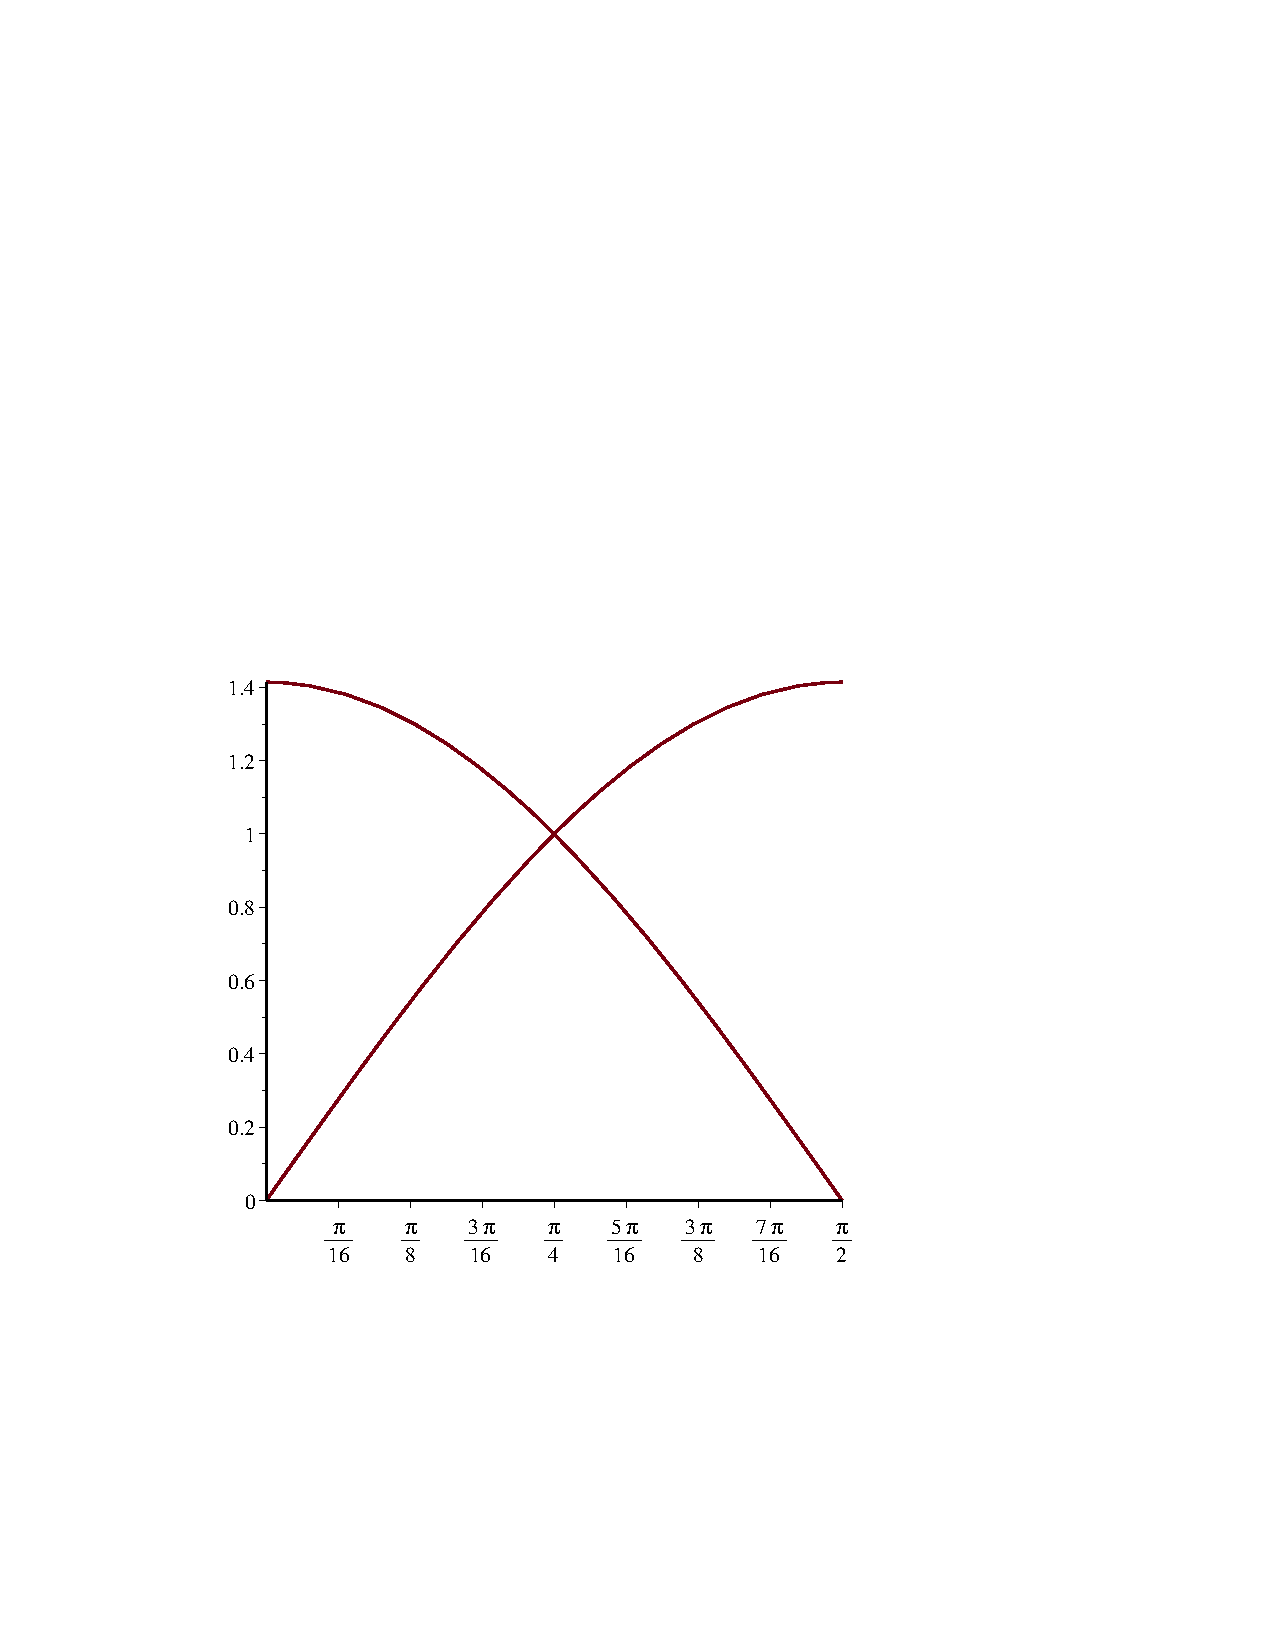
\includegraphics[scale=0.4]{graph.pdf}
\end{center}

Show that the graphs of $f(x)$ and $g(x)$ intersect at a right angle when $x=\frac{\pi}{4}$. (Hint: Show that the tangent lines to $f$ and $g$ at $x=\frac{\pi}{4}$ are perpendicular to each other.)

\includegraphics[scale=0.5]{start.pdf}
{{{1\linewidth}{$f^{\prime}\left(\frac{\pi}{4}\right)=-1$ and $g^{\prime}\left(\frac{\pi}{4}\right)=1$.  So, the tangent lines to $f$ and $g$ at $x=\frac{\pi}{4}$ are perpendicular to one another since the product of their slopes is $-1$.}}}
\includegraphics[scale=0.5]{end.pdf}


\newpage

\item A 15 foot ladder leans against a vertical wall at an angle of $\theta$ with the horizontal, as shown in the figure below.  The top of the ladder is $h$ feet above the ground.  If the ladder is pushed towards the wall, find the rate at which $h$ changes with respect to $\theta$ at the instant when $\theta=30^{\circ }$.  Express your answer in {\bf feet/degree}.

\begin{center}
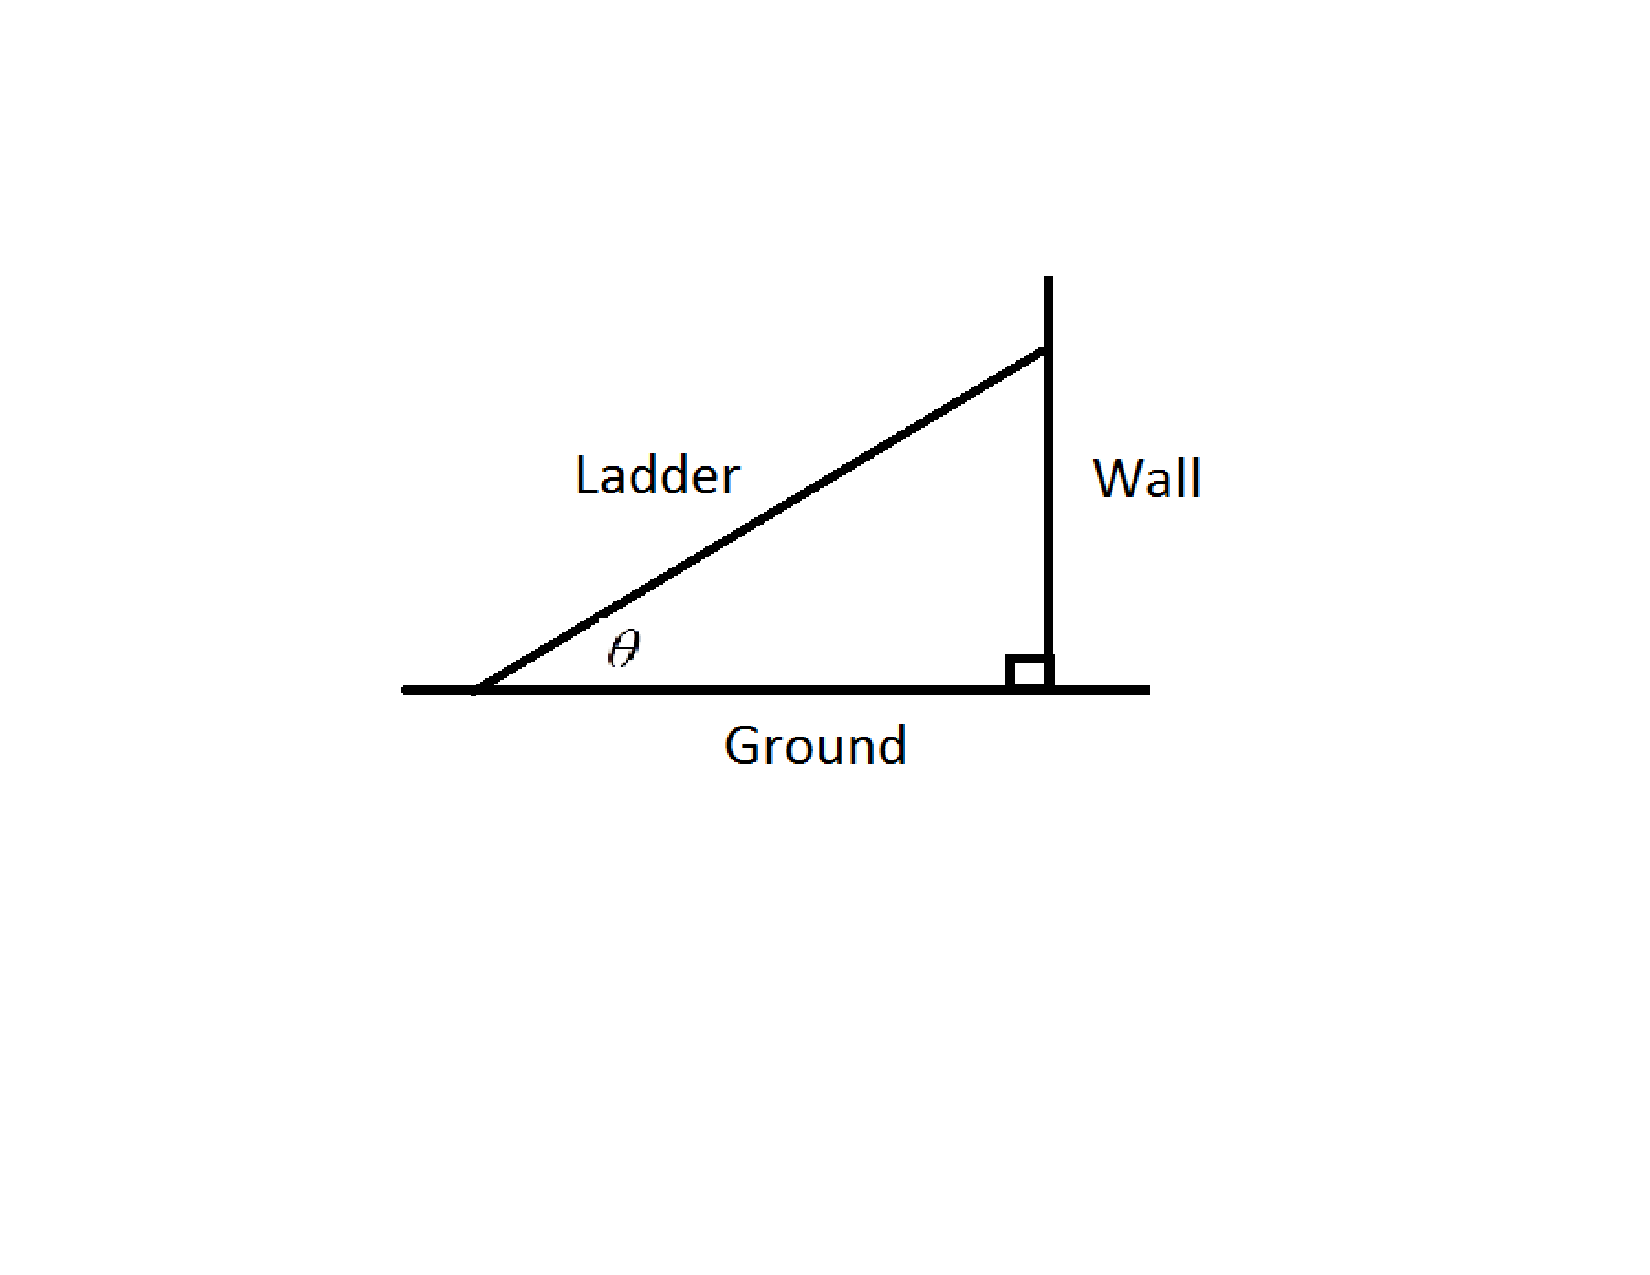
\includegraphics[scale=0.5]{wall.pdf}
\end{center}

\includegraphics[scale=0.5]{start.pdf}
{{$\frac{dh}{d\theta}=\frac{15\sqrt{3}}{2} \text{ ft/radian}=\frac{\pi\sqrt{3}}{24} \text{ ft/degree}$}}
\includegraphics[scale=0.5]{end.pdf}


\item Use the Intermediate Value Theorem to show that there is at least one point in the interval $(0,1)$ where the graph of $f(x)=\sin{x}-\frac{1}{3}x^3$ will have a horizontal tangent line.

\includegraphics[scale=0.5]{start.pdf}
{{{1\linewidth}{$f^{\prime}(x)=\cos{x}-x^2$.  Firstly, notice that $f^{\prime}(x)$ is continuous for all $x$; therefore, it is continuous for all $x$ in $[0,1]$.  Secondly, notice that $f^{\prime}(0)=1>0$ and $f^{\prime}(1)=\cos{(1)}-1<0$.  Thus, the Intermediate Value Theorem states there is at least one $x_0$ in the interval $(0,1)$ with $f^{\prime}(x_0)=0$.  In other words, there is at least one $x_0$ in $(0,1)$ where $f(x)$ will have a horizontal tangent line.}}}
\includegraphics[scale=0.5]{end.pdf}


\item {\bf Multiple Choice:} At how many points on the interval $[-\pi,\pi]$ is the tangent line to the graph of $y=2x+\sin{x}$ parallel to the secant line which passes through the graph endpoints of the interval?

\begin{enumerate}

\item 0

\item 1

\item 2

\item 3

\item None of these

\end{enumerate}

\includegraphics[scale=0.5]{start.pdf}
{{C}}
\includegraphics[scale=0.5]{end.pdf}


\end{enumerate}

\end{document}